%%%%%%%%%%%%%%%%%%%%%%%%%%%%%%%%%%%%%%%%%%%%%%%%%%%%%%%%%%%%%%%%%%%%%%%%%%%%%%%%
%2345678901234567890123456789012345678901234567890123456789012345678901234567890
%        1         2         3         4         5         6         7         8

%\documentclass[letterpaper, 10 pt, conference]{orbieeeconfpre}  % Comment this line out if you need a4paper

\documentclass[a4paper, 10pt, journal]{wissarbIEEE}      % Use this line for a4 paper
%\conference{IEEE Conference for Awesome ORB Research}

\bibliographystyle{orbref-num}

\IEEEoverridecommandlockouts                              % This command is only needed if 
                                                          % you want to use the \thanks command

\overrideIEEEmargins                                      % Needed to meet printer requirements.

% See the \addtolength command later in the file to balance the column lengths
% on the last page of the document

\usepackage{hyperref}
\usepackage{graphicx}
\usepackage{tabularx}
\usepackage{booktabs}
\usepackage{lipsum}
%von Max eingebunden:
%\usepackage{times}
\usepackage{url}
\usepackage{hyperref}
\usepackage{amsmath}              % Matheamtische Formeln
\usepackage{amsfonts}             % Mathematische Zeichensätze
\usepackage{amssymb}              % Mathematische Symbole
%\usepackage{underscore}

%% Wo sind die Bilder?
%\graphicspath{{bilder/}}


% Eigenes Makro für Bilder
\newcommand{\bild}[3]{
\begin{figure}[h]
\centering
  \includegraphics[width=#2]{#1}
  \caption{#3}
  \label{#1}
\end{figure}}

\newcommand{\length}[1]{\lvert \vec{#1} \rvert}

\title{\LARGE \bf
Automated conversion of CAD data in 3D low-poly models
}

\author{Dennis Becker}% <-this % stops a space

%\author{Maximilian Legnar$^{1}$ and Dr. Rasenat$^{2}$% <-this % stops a space
%
%\thanks{*Based on the guidelines published on the \href{http://conf.papercept.net/conferences/support/tex.php}{PaperCept conference manuscript management website}}% <-this % stops a space
%\thanks{$^{1}$Guybrush U. Threepwood is with the Institute for Pirate Sciences, Three-headed Monkey Group, University of  M\^el\'ee Island
%        {\tt\small gthreepwood@har.har-har.mi}}%
%\thanks{$^{2}$Alexander Schubert is with the Optimization in Robotics and Biomechanics Group, Institute of Computer Engineering, Heidelberg University, Berliner Str. 45, 69120 Heidelberg
%        {\tt\small alexander.schubert@ziti.uni-heidelberg.de, \href{http://orb.iwr.uni-heidelberg.de}{orb.iwr.uni-heidelberg.de}}}%
%}


\begin{document}

\maketitle

%%%%%%%%%%%%%%%%%%%%
\begin{abstract}

An automated conversion of CAD data into 3D low-poly models would offer great potential in the industrial environment. Automated transformation will allow companies to continue to use CAD models, which are already in existence. The converted models can be used, for example, in the field of virtual reality or even on mobile devices for high-performance and graphically appealing visualizations. This work addresses the question of how and in what quality such an automatic transformation is possible. By means of a prototypical implementation it is shown that such an automated conversion is possible and which problems occur.

\end{abstract}

\section{Low-Poly-models}
The topic and aim of this study are to investigate the extent to which existing CAD models can be fully automatically converted into high-performance and visually high-quality low-poly models. Low-poly-models are polygon (faces) meshes in 3D computer graphics, that has a relatively small number of polygons. However, as you can see in Figure 1, the optical quality of an object decreases significantly as the polygon number decreases. Round objects appear increasingly angular, many details are lost. In order to counteract this effect, numerous methods are used in game development to make low-poly models look high-quality. As many as possible of these methods should be used in the automatic conversion.

\bild{bilder/b1}{8.5cm}{ .. }

The created low poly models could be used for high quality realtime rendering, for example in industrial virtual reality applications. But also in the area of simulations, configurators or in mobile applications, the low-poly models could be used.

The creation of low-poly models is state of the art in the game industry. The low number of polygons and the associated low computational complexity allows almost photorealistic scenes in computer games to be rendered in real time \cite{unity}.  Here, however, the models are created manually by experienced artists. Although these models are accordingly very high quality, but also elaborate in their creation. It also requires extensive expertise for the manual creation of such models.

\section{automated conversion}
In contrast to this, software for the fully automatic conversion of CAD models could also be easily operated by laymen and would also be much faster. Thus, the automatic conversion could serve as the basis for high-performance 3D programs in the industrial and architectural sectors.

In order to examine this topic more closely, a concept was first worked out. The concept is based on the use of the open-source software Blender in combination with a specially developed Java control program.

To test the concept, a prototype implementation was made. The prototype can automatically convert polygon CAD models into low poly models. In the subsequent practical tests, the low-poly models not only had a significantly lower polygon count, but were also cleaned up for various possible sources of error. In this process, the metadata, for example the hierarchy of the CAD data, material settings and naming, can be adopted. In addition, the prototype shows some problems and limitations. Figures two and three show, by way of example, the CAD model of a turboshaft engine before and after the conversion. The corresponding parameters of the conversion can be found in Table 1. It shows that a polygon reduction of 90 \% and even more is possible. Also, display errors could be removed at the bottom of the model.

CAD-Modell: \hyperlink{https://grabcad.com/library/turbo-shaft-helicopter-engine-1}{https://grabcad.com/library/turbo-shaft-helicopter-engine-1} 

\bild{bilder/b2}{8cm}{ Turboshaft engine, 
cad-modell 1 }
\clearpage
\bild{bilder/b3}{8cm}{ Turboshaft engine, low-poly-modell }



\begin{table}[]
\caption{Vergleich Polygon-Modell und Low-Poly-Modell}
\label{my-label}
\begin{tabular}{llll}
\hline
                                      & Polygon-Model & Low-Poly-Model & Reduction \\ \hline
\multicolumn{1}{l|}{Polygons}         & 988.129       & 92.803         & 90,6 \%   \\
\multicolumn{1}{l|}{Vertices}         & 495.917       & 47.901         & 4,59 \%   \\
\multicolumn{1}{l|}{File size (.obj)} & 104 MB        & 5,48 MB        & 94,7 \%  
\end{tabular}
\end{table}


\section{Conclusion}

Overall, it can be said that an fast and easy automatic conversion of CAD data into high-quality low-poly models is possible. But it also turns out that automating low-poly techniques from game development is a big challenge. The developed prototype could serve as the basis for a comprehensive implementation in the future.


%%%%%%%%%%%%%%%%%%%%%%%%%%%%%%%%%%%%%%%%%%%%%%%%%%%%%%%%%%%%%%%%%%%%%%%%%%%%%%%%%
%\section{The short paper document class}
%{\bf Important!} Please note that the \verb!wissarbIEEE.cls! file is to be used within the context of the lecture {\it Wissenschaftliches Arbeiten} at the University Heidelberg only and must not be distributed externally!
%
%%% Figure
%\begin{figure}[h]
%   \centering
%   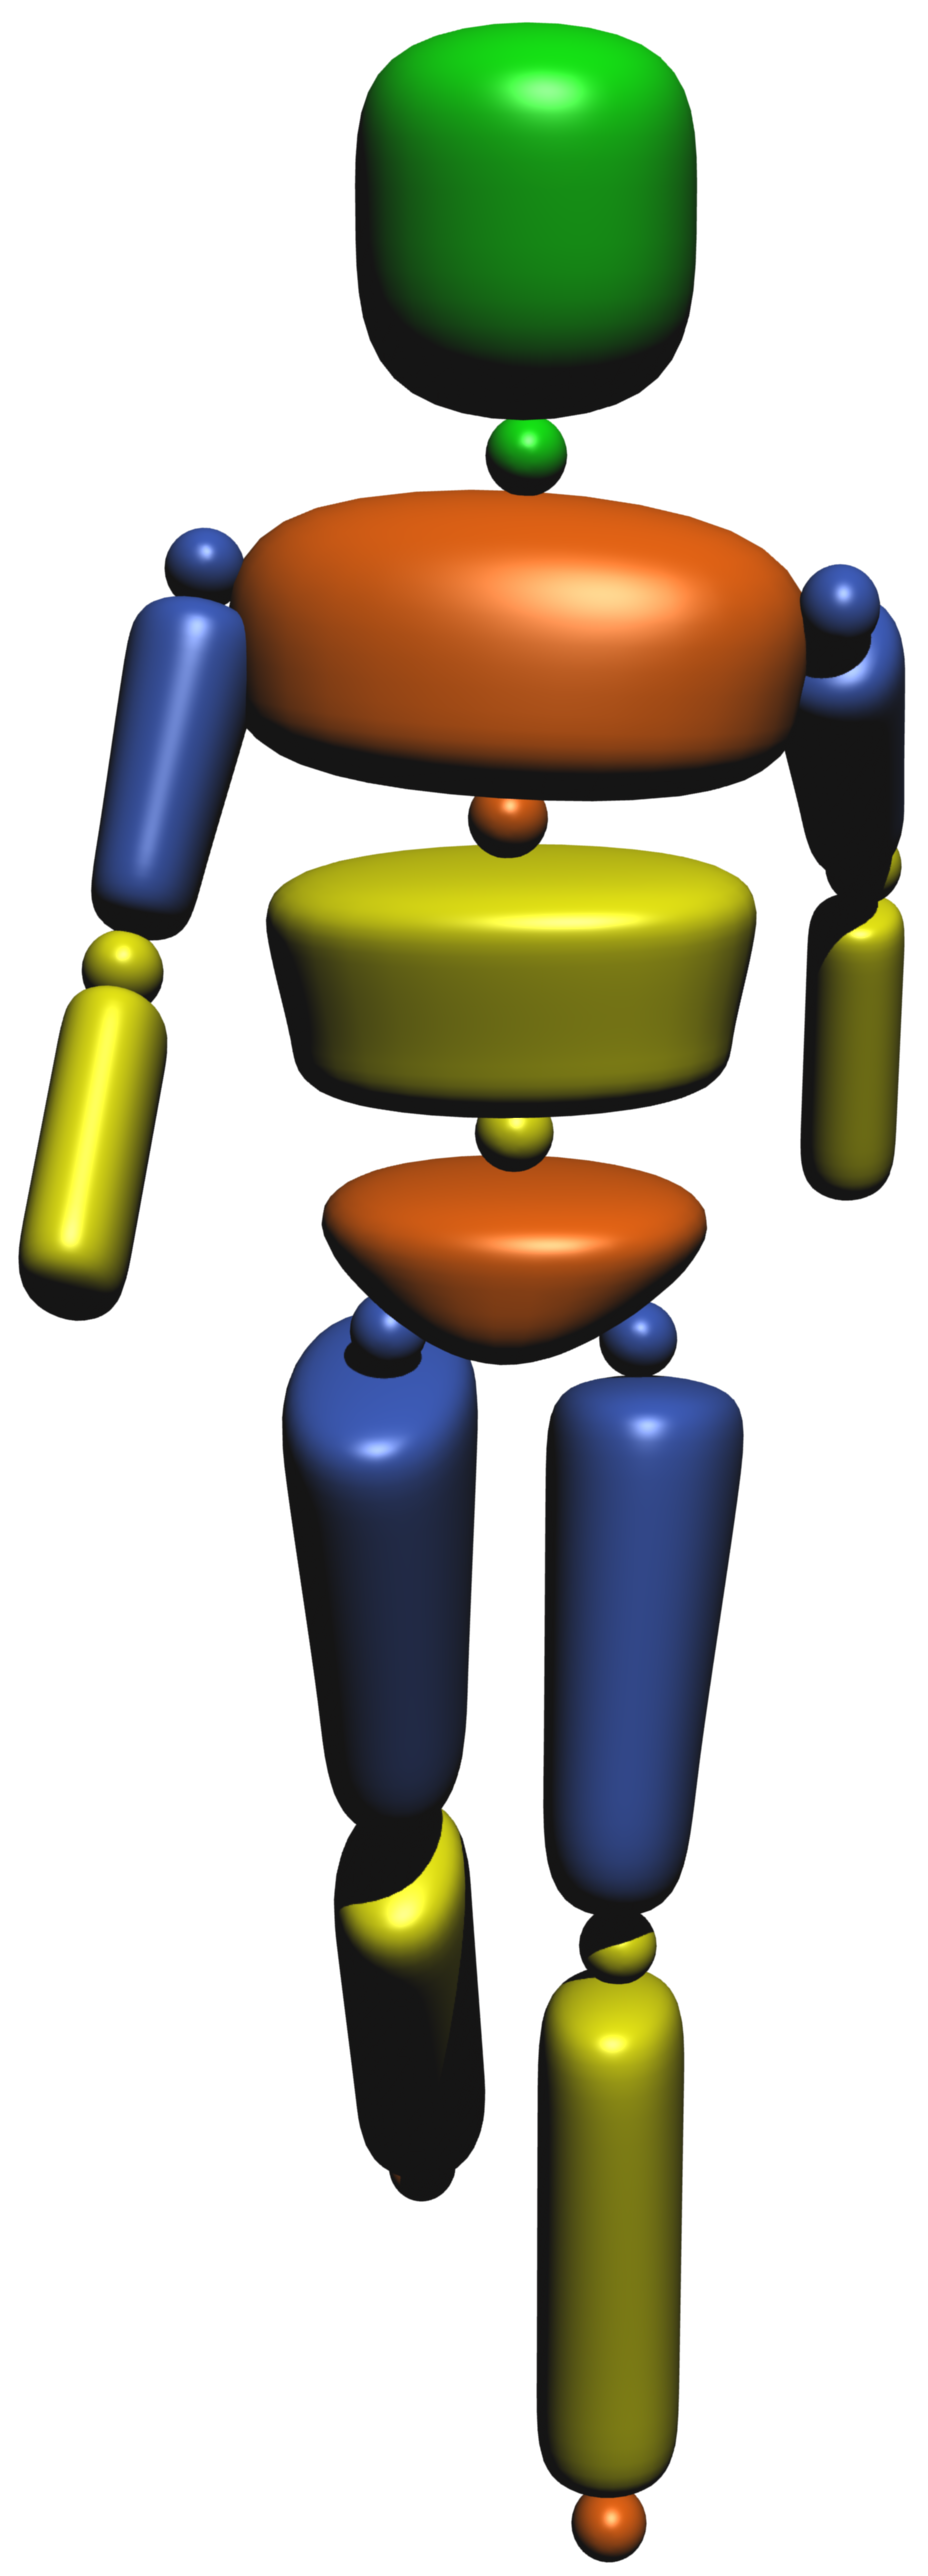
\includegraphics[width=0.1\textwidth]{fig/knubbi.png}
%   \caption{Example picture.}
%   \label{fig:knubbi}
%\end{figure}
%
%\subsection{Bibliography styles}
%The \texttt{orbref-num.bst} bibliography style numbers the citations by their order of appearance. Here are two sample references: \cite{Newton1687,Mombaur2009}.
%
%\subsection{Lorem Ipsum}
%\lipsum[1]
%
%%% Table
%\begin{table}[h]
%\caption{Vergleich Polygon-Modell und Low-Poly-Modell}
%   \begin{tabularx}{0.48\textwidth}{llr}
%   		 \toprule 
%   		 Symbol & \multicolumn{1}{X}{Description} & Value [m] \\
%		 \midrule
%		  $A_x$ & Horizontal coordinate of A$^{*}$ & 0.0745 \\
%		  $A_z$ & Vertical coordinate of A$^{*}$ & 0.2650 \\ 
%		  $C_x$ & Horizontal coordinate of C$^{\#}$ & 0.0700 \\
%		 \bottomrule
%   \end{tabularx}  \label{tab:initmodel}
%\end{table}
%
%\lipsum[2]

\bibliography{mybibfile}

\end{document}
